\chapter{Tetrahedral Quality Metrics}

All the metrics in this section are defined on a tetrahedral element with vertices
shown in Figure~\ref{f:tet}. Furthermore, we define the following edge vectors for
convenience
\begin{equation*}
\begin{array}{lcl}
\vec L_0 &=& \vec P_1 - \vec P_0\\
\vec L_1 &=& \vec P_2 - \vec P_1\\
\vec L_2 &=& \vec P_0 - \vec P_2
\end{array}\rule{10em}{0pt}
\begin{array}{lcl}
\vec L_3 &=& \vec P_3 - \vec P_0\\
\vec L_4 &=& \vec P_3 - \vec P_1\\
\vec L_5 &=& \vec P_3 - \vec P_2
\end{array}.
\end{equation*}

\begin{figure}[htb]
  \begin{center}
    \includegraphics[height=2.0in]{tet}
    \caption{Vertices of a tetrahedron.%
                                                                  \label{f:tet}}
  \end{center}
\end{figure}

The tetrahedron edge lengths are denoted as follows:
\[
L_0 = \normvec{L_0}\quad
L_1 = \normvec{L_1}\quad
L_2 = \normvec{L_2}\quad
L_3 = \normvec{L_3}\quad
L_4 = \normvec{L_4}\quad
L_5 = \normvec{L_5}
\]
and the largest and smallest edge lengths are, respectively,
\[
L_{\min} = \min\left(L_0, L_1, L_2, L_3, L_4, L_5\right)
  \rule{2em}{0pt}
L_{\max} = \max\left(L_0, L_1, L_2, L_3, L_4, L_5\right)
\]

The volume can then be defined in terms of the edge vectors as
\begin{equation*}
V = \frac{\left(\vec L_2\times\vec L_0\right)\cdot\vec L_3 }{6}.
\end{equation*}

In addition, we will respectively denote $R$ and $r$ the circumradius
and the inradius of the tetrahedron, \emph{i.e.}, respectively, the radii
of the circumscribed and inscribed spheres of this tetrahedron.
Note that the inradius is
\[
 r = \frac { 3V } { A }
\]
where $A$ is the  surface area of the tetrahedron:
\[
A = \frac{1}{2} \left(
      \normvec{L_2 \times \vec L_0} + 
      \normvec{L_3 \times \vec L_0} + 
      \normvec{L_4 \times \vec L_1} + 
      \normvec{L_3 \times \vec L_2}  \right),
\]
and that the the circumradius is
\[
 R = \frac {\Big\lVert
   \normvec{L_3}^2 \left( \vec L_2 \times \vec L_0 \right) + 
   \normvec{L_2}^2 \left( \vec L_3 \times \vec L_0 \right) + 
   \normvec{L_0}^2 \left( \vec L_3 \times \vec L_2 \right)
   \Big\rVert}{12 V }. 
\]

Sometimes, we will to refer to the edge vectors indexed by their endpoints:
\begin{equation*}
\begin{array}{lcl}
\vec L_{01} &=& \vec L_0\\
\vec L_{12} &=& \vec L_1\\
\vec L_{20} &=& \vec L_2
\end{array}\rule{10em}{0pt}
\begin{array}{lcl}
\vec L_{03} &=& \vec L_3\\
\vec L_{13} &=& \vec L_4\\
\vec L_{23} &=& \vec L_5
\end{array}
\end{equation*}

% -------------------Metric Table-------------------
\newcommand{\tetmetrictable}[8]{%
  \begin{center}
  \begin{tabular}{ll}
    \multicolumn{2}{r}{\textbf{\sffamily\Large tetrahedral #1}}\\\hline
    Dimension:                            & #2\\ 
    Acceptable Range:                     & #3\\ 
    Normal Range:                         & #4\\ 
    Full Range:                           & #5\\ 
    $q$ for unit equilateral tetrahedron: & #6\\
    Reference:                            & #7\\
    \verd\ function:       & \texttt{#8}\\ \hline
  \end{tabular} 
  \end{center}
}
\clearpage
\newpage %---------------------------Edge Ratio----------------------------------
\section{Edge Ratio}

The edge ratio of a tetrahedron is: 
\[
\frac{L_{\max}}{L_{\min}}.
\]

\tetmetrictable{edge ratio}%
{$1$}%                  Dimension
{$[1,3]$}%              Acceptable range
{$[1,DBL\_MAX]$}%       Normal range
{$[1,DBL\_MAX]$}%       Full range
{$1$}%                  Equilateral tet
{--}%                   Citation
{v\_tet\_edge\_ratio}%  Verdict function name


\newpage %---------------------------Aspect Beta----------------------------------
\section{Aspect Beta}

This metric measures the radius ratio (\emph{cf.}
\S\ref{s:tet-radius-ratio}) of a positively-oriented tetrahedron. Note
that it is equal to the tetrahedral radius ratio.

For a positively-oriented tetrahedron, the aspect $\beta$ is the
quotient of these two radii normalized by $\frac{1}{3}$ so 
that an equilateral tetrahedron has quality of~$1$:
\begin{eqnarray*}
q & = & \frac{R}{3 r} \nonumber \\
  & = & \frac { \left| 
   \normvec{L_3}^2 \left( \vec L_2 \times \vec L_0 \right) + 
   \normvec{L_2}^2 \left( \vec L_3 \times \vec L_0 \right) + 
   \normvec{L_0}^2 \left( \vec L_3 \times \vec L_2 \right)
   \right| A}{108 V^2}.
\end{eqnarray*}

Note that if the tetrahedron has negative orientation, we set $q = DBL\_MAX$.

\tetmetrictable{aspect $\beta$}%
{$1$}%                  Dimension
{$[1,3]$}%              Acceptable range
{$[1,DBL\_MAX]$}%       Normal range
{$[1,DBL\_MAX]$}%       Full range
{$1$}%                  Equilateral tet
{\cite{par:93}}%        Citation
{v\_tet\_aspect\_beta}% Verdict function name

\newpage %-------------------------------Aspect Delta---------------------------------
\section{Aspect Delta}

Aspect $\delta$ is a dimensionless number defined as the smallest ratio of the
height of a vertex above its opposing triangle (see Figure~\ref{f:tet-height}) to
the square root of the area the triangle across all vertices of the tetrahedron. 
\begin{figure}[bhp]
  \centering
  \includegraphics[width=1.5in]{tet-height}
  \caption{
    An illustration of the height $h_3$ of vertex 3.%
                                                          \label{f:tet-height}}
\end{figure}
In general, take $(i,j,k,\ell)$ to be a permutation of $\{0,1,2,3\}$
(i.e., $(i,j,k,\ell)\in\Sf$) and $\normvec{ L_{ab}}$ to be the length of the edge
connecting vertices $a$ and $b$.
Then aspect ratio $\delta$ may be written
\[
  q = \min_i\left\{C\frac{h_i}{\sqrt{A_{jk\ell}}}\right\}
\]
where $A_{jk\ell}$ is the area of the triangle opposite vertex $i$ and
$C = \frac{\sqrt[4]{108}}{4}\approx 0.805927$ chosen so that an equilateral tetrahedron has $q = 1$.
PATRAN~\cite{patran:03} also speaks of a ``normalized'' aspect ratio defined as
\[
  q_{alt} = 1 - q = 1 - \min_i\left\{C\frac{h_i}{\sqrt{A_{jk\ell}}}\right\}
\]
which is 0 for an equilateral tetrahedron.

\tetmetrictable{aspect $\delta$}%
{$1$}%                                                Dimension
{$[0.1,DBL\_MAX]$}%                                   Acceptable range
{$(0,DBL\_MAX]$}%                                     Normal range
{$[0,DBL\_MAX]$}%                                     Full range
{$1$}%                                                Equilateral tet
{\cite{patran:03}}%                                   Citation
{\nsup}%                                              Verdict function name



\newpage %---------------------------Aspect Frobenius-----------------------------
\section{Aspect Frobenius\label{s:tet-aspect-Frobenius}}

The edge matrix of the tetrahedral element is defined as
follows:
\[
T_0 = (\vec{L_0}\;\vec{L_1}\;\vec{L_2})
\]
and let $W$ be the edge matrix of the reference regular tetrahedron.
Consider the matrix that maps $W$ into $T_0$:
\[
A_0 = T_0 W^{-1}.
\]
The Frobenius norm of $A_0$ is
\[
|A_0|_F = \sqrt{\mathrm{tr}(A_0^T\, A_0)},
\]
and the Frobenius condition number is the condition number associated
with this norm.

The aspect Frobenius of the element is defined as the normalized
(equal to $1$ when the element is regular) Frobenius condition number of $A_0$.

\tetmetrictable{aspect Frobenius}%
{$1$}%                                                Dimension
{$[1,1.3]$}%                                          Acceptable range
{$[1,DBL\_MAX]$}%                                     Normal range
{$[1,DBL\_MAX]$}%                                     Full range
{$1$}%                                                Unit equilateral triangle value
{\cite{knu:00}}%                                      Reference(s)                   
{v\_tet\_aspect\_frobenius}%                            Verdict function name

\newpage %---------------------------Aspect Gamma-----------------------------
\section{Aspect Gamma}

This metric compares root-mean-square edge length to volume.
The root-mean-square edge length is
\[
R = \sqrt{\frac{\sum_{i=0}^{5}\normvec{L_i}^2}{6}}
\]
and so, normalizing the metric to a value of 1 for equilateral tetrahedra, we have
\[
q = \frac{R^3\sqrt{2}}{12|V|}.
\]

Note that if  $|V| < DBL\_MIN$, we set $q = DBL\_MAX$.

\tetmetrictable{aspect $\gamma$}%
{$1$}%                  Dimension
{$[1,3]$}%              Acceptable range
{$[1,DBL\_MAX]$}%       Normal range
{$[1,DBL\_MAX]$}%       Full range
{$1$}%                  Equilateral tet
{\cite{par:93}}%        Citation
{v\_tet\_aspect\_gamma}%                            Verdict function name


\newpage %---------------------------Aspect Ratio----------------------------------
\section{Aspect Ratio\label{s:tet-aspect-ratio}}

The aspect ratio of a tetrahedron $K$ is: 
\[
\frac{L_{\max}}{2\sqrt{6}r}.
\]

\tetmetrictable{aspect ratio}%
{$1$}%                  Dimension
{$[1,3]$}%              Acceptable range
{$[1,DBL\_MAX]$}%       Normal range
{$[1,DBL\_MAX]$}%       Full range
{$1$}%                  Equilateral tet
{\cite{frey:00}}%        Citation
{v\_tet\_aspect\_ratio}%                            Verdict function name

\newpage %-------------------------------Collapse Ratio---------------------------------
\section{Collapse Ratio}

The collapse ratio is a dimensionless number defined as the smallest ratio of the
height of a vertex above its opposing triangle to the longest edge of that opposing
triangle across all vertices of the tetrahedron. Figure~\ref{f:tet-height} shows
how the ratio is computed for a single vertex (vertex $3$). Assuming that edge $0-2$
is the longest edge of triangle $0-1-2$, the collapse ratio for vertex $3$ becomes:
\[
  q_{ex} = \frac{h_3}{\normvec{ L_{02}}}.
\]
In general, take $(i,j,k,\ell)$ to be a permutation of $\{0,1,2,3\}$
(i.e., $(i,j,k,\ell)\in\Sf$) and $\normvec{ L_{ab}}$ to be the length of the edge
connecting vertices $a$ and $b$.
Then the collapse ratio may be written
\[
  q = \min_i\left\{\frac{h_i}{\max\left\{\normvec{ L_{jk}},\normvec{ L_{k\ell}},\normvec{ L_{\ell j}}\right\}}\right\}.
\]

The collapse ratio is intended to identify tetrahedra whose vertices are nearly planar (slivers).
Note that $q$ approaches zero as vertex $3$ in
Figure~\ref{f:tet-height} approaches the plane defined by $0-1-2$.
However, this metric can be misleading when the vertex with the smallest projected height
(say $3$ without loss of generality) is not projected interior to triangle $0-1-2$.
In this case, it is possible for $0-1-2$ to have a small area (which increases $q$) but
for edges $0-3$, $1-3$, and $2-3$ to be very long compared to those of triangle $0-1-2$.
Thus slivers can have arbitrarily high collapse ratios.

\tetmetrictable{collapse ratio}%
{$1$}%                                                Dimension
{$[0.1,DBL\_MAX]$}%                                   Acceptable range
{$(0,DBL\_MAX]$}%                                     Normal range
{$[0,DBL\_MAX]$}%                                     Full range
{$\frac{\sqrt{6}}{3}$}%                               Equilateral tet
{\cite{patran:03}}%                                   Citation
{v\_tet\_collapse\_ratio}%                            Verdict function name



\newpage %---------------------------Condition-----------------------------
\section{Condition}

First, define
\[
\begin{array}{lcl}
\vec C_1 &=& \vec L_0 \\
\vec C_2 &=& \left(-2 \vec L_2 - \vec L_0\right)/\sqrt{3} \\
\vec C_3 &=& \left(3 \vec L_3 + \vec L_2 - \vec L_0\right)/\sqrt{6}
\end{array}
\]
\[
C_{det} = \vec C_1 \cdot ( \vec C_2 \times \vec C_3 ),
\]

and
\[
\begin{array}{lcl}
T_1 &=& \vec C_1 \cdot \vec C_1 + \vec C_2 \cdot \vec C_2 + \vec C_3 \cdot \vec C_3\\
T_2 &=& (\vec C_1 \times \vec C_2 ) \cdot (\vec C_1 \times \vec C_2) + 
      (\vec C_2 \times \vec C_3 ) \cdot (\vec C_2 \times \vec C_3) + 
      (\vec C_1 \times \vec C_3 ) \cdot (\vec C_1 \times \vec C_3)
\end{array}
\]

The condition metric is then defined as follows:
\begin{equation*}
q = \frac{ \sqrt{ T_1 T_2 } } { 3 C_{det} }.
\end{equation*}

Note that if If $C_{det} \leq DBL\_MIN$, we set $q = DBL\_MAX$.

\tetmetrictable{condition}%
{$1$}%                  Dimension
{$[1,3]$}%              Acceptable range
{$[1,DBL\_MAX]$}%       Normal range
{$[1,DBL\_MAX]$}%       Full range
{$1$}%                  Equilateral tet
{\cite{knu:00}}%        Citation
{v\_tet\_condition}%                            Verdict function name



\newpage %---------------------------Distortion---------------------------
\section{Distortion}

The distortion is a measure of how well-behaved the mapping from
parameter space to world coordinates is.
The parameter space is defined using a ``master'' tetrahedron
with vertices
\[
\begin{array}{lcrcrcrc}
 \vec P_0 &= (& -1&,& -\frac{ \sqrt{3}}{3}&,& -\frac{2\sqrt{6}}{9}&)\\
 \vec P_1 &= (&  1&,& -\frac{ \sqrt{3}}{3}&,& -\frac{2\sqrt{6}}{9}&)\\
 \vec P_2 &= (&  0&,&  \frac{2\sqrt{3}}{3}&,& -\frac{2\sqrt{6}}{9}&)\\
 \vec P_3 &= (&  0&,&                    0&,&  \frac{4\sqrt{6}}{9}&)
\end{array}
\]
and volume $V_m$.
The behavior of the map is measured by sampling the determinant of the
Jacobian at Gauss points $G = \{g_k\}$.
The minimum of these is then used to scale the ratio of the
``master'' tetrahedron to the tetrahedron of interest:
\[
q = \frac{\min_k\{\det(J_{g_k})\} V_m}{V}
\]

Note that if $V < DBL\_MIN$, we set $q = DBL\_MAX$.
This metric is currently unsupported.

\tetmetrictable{distortion}%
{$1$}%                          Dimension
{$[0.5,1]$}%                    Acceptable range
{$[0,1]$}%                      Normal range
{$[-DBL\_MAX,DBL\_MAX]$}%       Full range
{$0$}%                          Equilateral tet
{Adapted from \cite{ideas:xx}}% Citation
{v\_tet\_distortion}%                            Verdict function name


\newpage %---------------------------Jacobian-----------------------------
\section{Jacobian\label{s:tet-jacobian}}

This metric is defined as follows:
\begin{displaymath}
q = \left( \vec L_2 \times \vec L_0 \right) \cdot \vec L_3  
\end{displaymath}

\tetmetrictable{Jacobian}%
{$L^3$}%                  Dimension
{$[0,DBL\_MAX]$}%         Acceptable range
{$[0,DBL\_MAX]$}%         Normal range
{$[-DBL\_MAX,DBL\_MAX]$}% Full range
{$\frac{\sqrt{2}}{2}$}%   Equilateral tet
{\cite{knu:03}}%          Citation
{v\_tet\_jacobian}%                            Verdict function name


\newpage %---------------------------Minimum Angle-----------------------------
\section{Minimum Angle\label{s:tet-min-angle}}

The (nonoriented) dihedral angle of two faces of the
tetrahedron that are adjacent along edge $i$ ($0\le{}i\le5$), is,
measured in degrees,
\[
  \alpha_i = \frac{180\dgr}{\pi}
    \arccos{\left(\vec{n_{i1}} \cdot \vec{n_{i2}}\right)},
\]
where $\vec{n_{i1}}$ and $\vec{n_{i2}}$ are unit vectors normal to the
two tetrahedron faces that are adjacent to edge $i$. Subsequently,
the minimum (nonoriented) dihedral angle of the tetrahedron, measured
in degrees, is
\[
  q =
    \min_{i\in\{0,1,2,3,4,5\}}{\alpha_i}.
\]

\tetmetrictable{minimum dihedral angle}%
{$A^1$}%                                              Dimension
{$[40\dgr,\frac{180\dgr}{\pi}\arccos\tfrac{1}{3}]$}%  Acceptable range
{$[0\dgr,\frac{180\dgr}{\pi}\arccos\tfrac{1}{3}]$}%   Normal range
{$[0\dgr,360\dgr]$}%                                  Full range
{$\frac{180\dgr}{\pi}\arccos\tfrac{1}{3}\approx70.528779\dgr$}% Regular tetrahedron value
{--}%                                                 Reference(s)                   
{v\_tet\_minimum\_angle}%                             Verdict function name


\newpage %---------------------------Radius Ratio----------------------------------
\section{Radius Ratio\label{s:tet-radius-ratio}}

This metric is commonly known as the radius ratio since it is the
normalized ratio of the radius of the inscribed sphere to the radius
of the circumsphere. Note that it is equal to the tetrahedral aspect
$\beta$ for positively-oriented tetrahedra.  

The radius ratio is the quotient of these two radii normalized by $\frac{1}{3}$ so
that an equilateral tetrahedron has quality of 1:
\begin{eqnarray*}
q & = & \frac{R}{3 r} \nonumber \\
  & = & \frac { \left| 
   \normvec{L_3}^2 \left( \vec L_2 \times \vec L_0 \right) + 
   \normvec{L_2}^2 \left( \vec L_3 \times \vec L_0 \right) + 
   \normvec{L_0}^2 \left( \vec L_3 \times \vec L_2 \right)
   \right| A}{108 V^2}.
\end{eqnarray*}

Note that if $|V| < DBL\_MIN$, we set $q = DBL\_MAX$.

\tetmetrictable{radius ratio}%
{$1$}%                  Dimension
{$[1,3]$}%              Acceptable range
{$[1,DBL\_MAX]$}%       Normal range
{$[1,DBL\_MAX]$}%       Full range
{$1$}%                  Equilateral tet
{\cite{par:93}}%        Citation
{v\_tet\_radius\_ratio}% Verdict function name



\newpage %---------------------------Relative Size-----------------------------
\section{Relative Size Squared\label{s:tet-rel-size-squared}}

This metric measures the size of a tetrahedron relative to an ensemble
containing it using volume.
Take $\overline{V}$ to be the average volume of the tetrahedra in the ensemble being analyzed
and define
\[
R = \frac{V}{\overline{V}}
\]
Then the quality is defined as
\begin{equation*}
q =  \left[ \min\left( R, \frac {1}{R}\right) \right]^2.
\end{equation*}

Note that if $\overline{V} < DBL\_MIN$ or if $R \leq DBL\_MIN$, we set $q = 0$.

\tetmetrictable{relative size squared}%
{$1$}%                  Dimension
{$[0.3,1]$}%            Acceptable range
{$[0,1]$}%              Normal range
{$[0,1]$}%              Full range
{N/A}%                  Equilateral tet
{\cite{knu:03}}%        Citation
{v\_tet\_relative\_size\_squared}%                            Verdict function name


\newpage %---------------------------Scaled Jacobian-----------------------------
\section{Scaled Jacobian}

Let $J$ be the Jacobian as defined in \S\ref{s:tet-jacobian}

\[
\lambda_1 = \normvec{ L_0 }
            \normvec{ L_2 }
            \normvec{ L_3 }  
\]

\[
\lambda_2 = \normvec{ L_0 }
            \normvec{ L_1 }
            \normvec{ L_4 }  
\]

\[
\lambda_3 = \normvec{ L_1 }
            \normvec{ L_2 }
            \normvec{ L_5 }  
\]

\[
\lambda_4 = \normvec{ L_3 }
            \normvec{ L_4 }
            \normvec{ L_5 }  
\]


\[
\lambda_{\max} = \max\left\{\lambda_1, \lambda_2, \lambda_3, \lambda_4, J\right\} 
\]

\begin{equation*}
q = \frac{J\sqrt{2}}{\lambda_{\max}}
\end{equation*}

Note that if $\lambda_{\max} < DBL\_MIN$, we set $q = DBL\_MAX$.

\tetmetrictable{scaled Jacobian}%
{$1$}%                                        Dimension
{$[\frac{1}{2},\frac{\sqrt{2}}{2}]$}%         Acceptable range
{$[-\frac{\sqrt{2}}{2},\frac{\sqrt{2}}{2}]$}% Normal range
{$[-DBL\_MAX,DBL\_MAX]$}%                     Full range
{1}%                                          Equilateral tet
{\cite{knu:00}}%                              Citation
{v\_tet\_scaled\_jacobian}%                            Verdict function name


\newpage %---------------------------Shape-----------------------------
\section{Shape\label{s:tet-shape}}

Let $J$ be the Jacobian as defined in \S\ref{s:tet-jacobian}.
We define the shape quality metric as
\begin{equation*}
q =  \frac{ 3 \left( J \sqrt{2} \right)^{2/3} } 
              { \frac {3}{2} \left( 
                      \vec L_0 \cdot  \vec L_0 +
                      \vec L_2 \cdot  \vec L_2 +
                      \vec L_3 \cdot  \vec L_3  \right) - 
               \left( \vec L_0 \cdot -\vec L_2 +
                      \vec L_0 \cdot  \vec L_3 +
                     -\vec L_2 \cdot  \vec L_3 \right) } 
\end{equation*}

Note that if $J < DBL\_MIN$, $q = 0$.
If $\frac {3}{2} \left( \vec L_0 \cdot \vec L_0 +
                      \vec L_2 \cdot \vec L_2 +
                      \vec L_3 \cdot \vec L_3  \right) - 
                 \left( \vec L_0 \cdot -\vec L_2 +
                      \vec L_0 \cdot \vec L_3 +
                      -\vec L_2 \cdot \vec L_3 \right) < DBL\_MIN$, we set $q = 0$.

\tetmetrictable{shape}%
{$1$}%                                        Dimension
{$[0.3,1]$}%                                  Acceptable range
{$[0,1]$}%                                    Normal range
{$[0,1]$}%                                    Full range
{1}%                                          Equilateral tet
{\cite{knu:03}}%                              Citation
{v\_tet\_shape}%                            Verdict function name



\newpage %---------------------------Shape and Size-----------------------------
\section{Shape and Size\label{s:tet-shape-and-size}}

Let $S$ be the shape as defined in \S\ref{s:tet-shape}
and $R$ be the relative size squared as defined in \S\ref{s:tet-rel-size-squared}.
Then the shape and size metric is
\begin{displaymath}
q = S R
\end{displaymath}

\tetmetrictable{shape and size}%
{$1$}%                                        Dimension
{$[0.2,1]$}%                                  Acceptable range
{$[0,1]$}%                                    Normal range
{$[0,1]$}%                                    Full range
{Dependent on $\overline{V}$}%                Equilateral tet
{\cite{knu:03}}%                              Citation
{v\_tet\_shape\_and\_size}%                            Verdict function name


\newpage %---------------------------Volume-----------------------------
\section{Volume}

The tetrahedron volume metric is simply
\[
q = V.
\]

\tetmetrictable{volume}%
{$L^3$}%                                      Dimension
{$[0,DBL\_MAX]$}%                             Acceptable range
{$[-DBL\_MAX,DBL\_MAX]$}%                     Normal range
{$[-DBL\_MAX,DBL\_MAX]$}%                     Full range
{$\frac { \sqrt{2}} {12}$}%                   Equilateral tet
{\cite{par:93}}%                              Citation
{v\_tet\_volume}%                            Verdict function name

